\section{Partie commande d'une GTB}

La commande d'une GTB est assurée par un automate programmable industriel (API). Cet automate est un ordinateur industriel programmable. Il est capable de communiquer avec les différents équipements du bâtiment (capteurs, actionneurs, superviseur, etc.) par l'intermédiaire de BUS de terrain. 

\subsection{Automate programmés et automates programmables}
Les constructeurs d'automates proposent des structures de commande spécifiques à certains domaines d'activité. Ces automates sont appelés automates programmés. Ils doivent être configurés pour mise en service. Ils ne sont pas programmables.\\

Les automates programmables sont des ordinateurs industriels programmables. Ils sont capables de communiquer avec les différents équipements du bâtiment (capteurs, actionneurs, superviseur, etc.) par l'intermédiaire de BUS de terrain.
Ceux-ci sont programmables et donc plus versatiles. 

Les constructeurs fournissent des bibliothèques de fonctions permettant de gérer les différents BUS de terrain.

\subsection{Rappel : Le cycle automate}

\begin{minipage}{0.55\linewidth}
Quelques caractéristiques du système d'exploitation d'un automate :
\begin{itemize}
    \item Temps réel (chien de garde)
    \item Déterministe
    \item Interruptible
    \item Monotâche ou Multitâches 
    \item Accès facilités aux entrées/sorties
    \item Accès facilités à la mémoire
\end{itemize}
\end{minipage}
\begin{minipage}{0.4\linewidth}
    \begin{UPSTIactivite}[][Cycle automate]
        \UPSTIeleveOnly{\vspace{7cm}}
        \UPSTIprofOnly{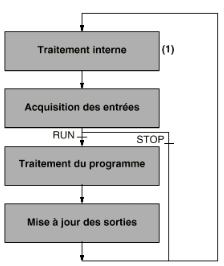
\includegraphics[height=6.5cm]{cycleAutomate}}
    \end{UPSTIactivite}
\end{minipage}
